\documentclass[11pt,rgb,ratio=169]{beamer}
\usetheme[nologo,vier,talk]{Wuppertal}
\usepackage[utf8]{inputenc}
\usepackage[T1]{fontenc}
\usepackage{lmodern}
\usepackage{amsmath,amssymb,mathtools}
\usepackage{graphicx}
\usepackage{booktabs}
\usepackage{xcolor}
\usepackage{array}
\usepackage{tikz}
\usepackage{ragged2e}
\beamertemplatenavigationsymbolsempty
\setbeamertemplate{headline}{}
\setbeamertemplate{logo}{}
\setbeamersize{text margin left=8mm,text margin right=8mm}
\setlength{\abovedisplayskip}{0.35em}
\setlength{\belowdisplayskip}{0.35em}

\newif\ifbackupslide
\backupslidefalse

% BUW green, close to the university logo green
\definecolor{BUWgreen}{RGB}{151,193,27}
\definecolor{BUWdarkgreen}{RGB}{129,171,45}

\setbeamercolor{ma footer left}{bg=BUWdarkgreen,fg=white}
\setbeamercolor{ma footer mid}{bg=BUWdarkgreen,fg=white}
\setbeamercolor{ma footer logo}{bg=BUWgreen,fg=white}

% Compact BUW-green footer with logo on every slide.
\setbeamertemplate{footline}{%
  \leavevmode%
  \hbox{%
  \begin{beamercolorbox}[wd=.72\paperwidth,ht=2.7ex,dp=1.0ex,leftskip=1em]{ma footer left}%
    \scriptsize Dhruv Patel \;--\; Laplace-static flux-tube profiles%
  \end{beamercolorbox}%
\begin{beamercolorbox}[wd=.13\paperwidth,ht=2.7ex,dp=1.0ex,rightskip=.7em]{ma footer mid}%
  \hfill\scriptsize
  \ifbackupslide
    Backup
  \else
    \insertframenumber/\inserttotalframenumber
  \fi
\end{beamercolorbox}%
  \begin{beamercolorbox}[wd=.15\paperwidth,ht=2.7ex,dp=1.0ex,center]{ma footer logo}%
    \raisebox{-0.35ex}{
\includegraphics[height=2.15ex]{buw-logo-white.pdf}}%
  \end{beamercolorbox}}%
}

\title[Laplace-static flux-tube project]{Laplacian-Eigenmode Static Sources to Gluonic Flux-Tube Profiles}
\author{Dhruv Patel}
\institute{Bergische Universit\"at Wuppertal}
\date{25 June 2026}

\newcommand{\smallcite}[1]{{\scriptsize\textcolor{gray!80!black}{#1}}}
\newcommand{\good}[1]{\textcolor{WtalFakVierGruen}{#1}}
\newcommand{\warn}[1]{\textcolor{orange!85!black}{#1}}
\newcommand{\diag}[1]{\textcolor{gray!85!black}{#1}}
\newcommand{\tightitems}{\setlength\itemsep{0.28em}\setlength\parskip{0pt}}
\newcommand{\eqbox}[1]{\begin{center}\fcolorbox{WtalFakVierBlau}{gray!5}{\begin{minipage}{0.94\linewidth}#1\end{minipage}}\end{center}}

\begin{document}
\maketitle

% ------------------------------------------------------------------
\begin{frame}{Project aim: from static potential to gluonic flux-tube profiles}

\begin{columns}[T,totalwidth=\textwidth]
% ------------------------------------------------------------
\begin{column}{0.50\textwidth}
\textbf{Physics target}\vspace{0.25em}

\begin{itemize}\tightitems
  \item Build static $Q\bar Q$ sources with Laplacian-eigenmode trial states.
  \item Validate via a static-potential benchmark.
  \item Then insert local gluonic probes to map the flux tube.
\end{itemize}

\vspace{0.6em}
\textbf{Gluonic probe: action density}

\vspace{-0.25em}
{\scriptsize
\begin{align*}
S(\vec z,t)
&=
\frac12\left(E^2(\vec z,t)+B^2(\vec z,t)\right), \\[0.45em]
\Delta S_{Q\bar Q}(\vec z;R,\tau)
&=
\frac{
\left\langle L(R,\tau)\,S(\vec z,t_{\rm mid})\right\rangle
}{
\left\langle L(R,\tau)\right\rangle
}
-
\left\langle S(\vec z,t_{\rm mid})\right\rangle .
\end{align*}
}
\end{column}

% ------------------------------------------------------------
\begin{column}{0.46\textwidth}
\centering
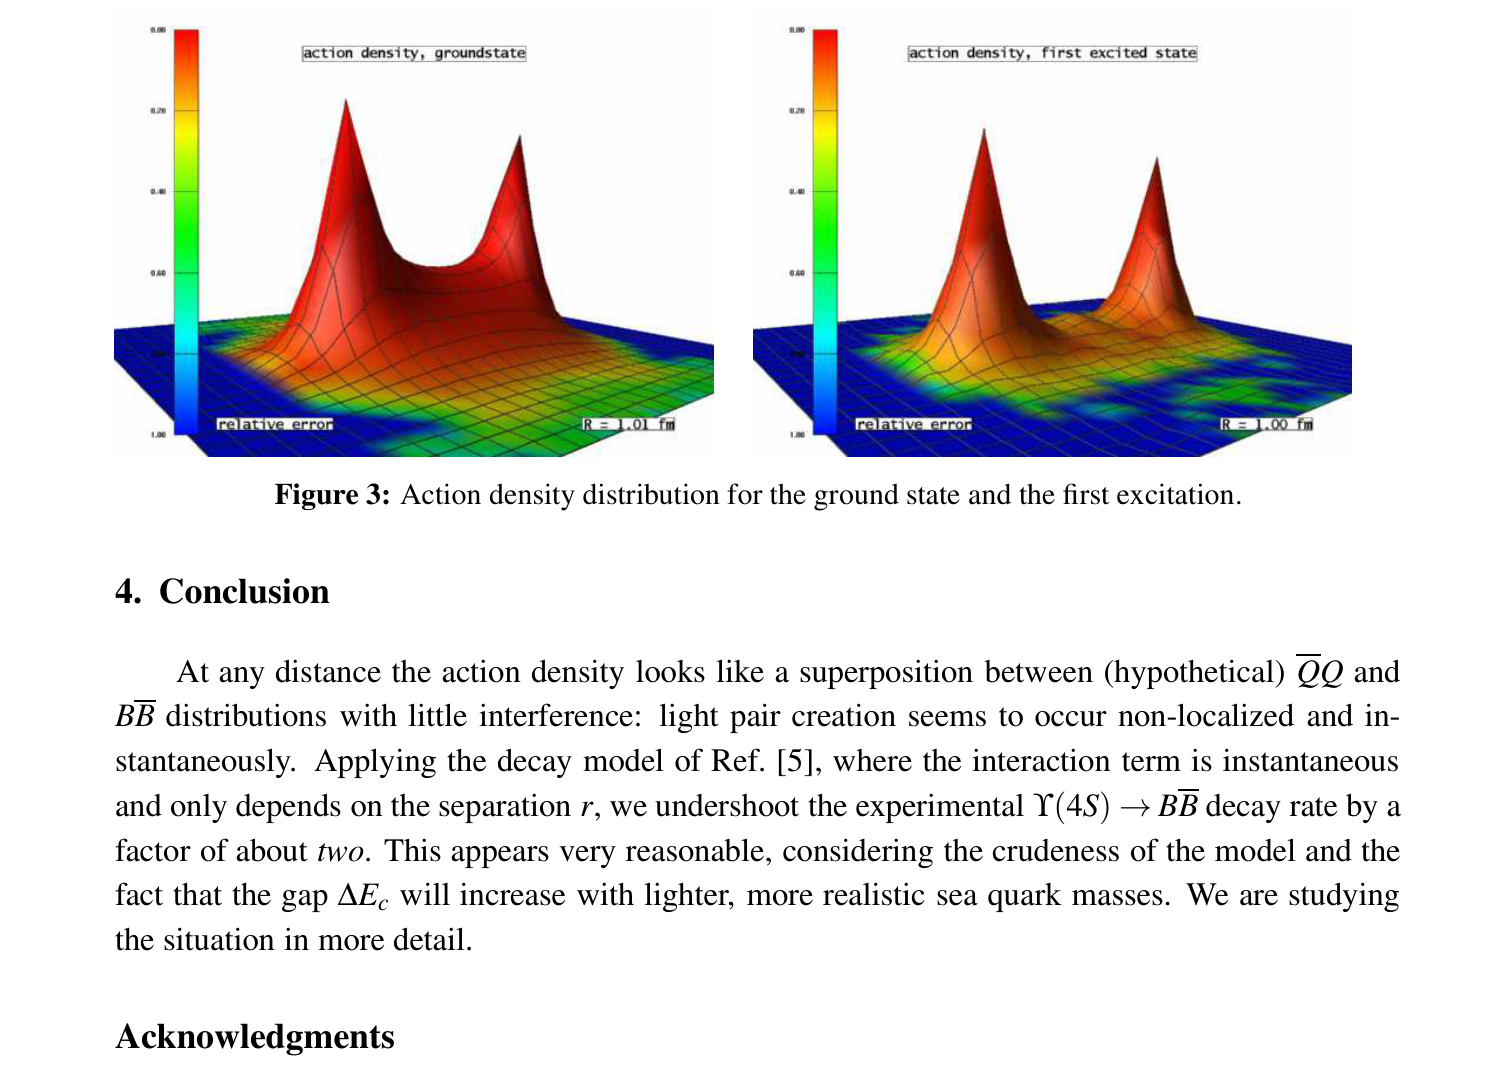
\includegraphics[height=0.32\textheight,width=0.96\linewidth,keepaspectratio]{bali_action_density_fig3.png}

\vspace{0.25em}
\smallcite{Flux-tube/string-breaking paper: Bali et al., PoS LAT2005 (2005).}

\vspace{1.23em}
\hspace*{0.03\linewidth}%
\begin{beamercolorbox}[rounded=true,sep=0.55em,wd=0.75\linewidth]{block body}
\centering
\small
Given a static quark and antiquark separated by $R$,\\
how is the gluonic field modified at the point $\vec z$\,?
\end{beamercolorbox}
\end{column}
\end{columns}

\end{frame}

% ------------------------------------------------------------------
\begin{frame}{Methodology and resources used in the project}
\begin{columns}[T,totalwidth=\textwidth]
\begin{column}{0.50\textwidth}
\textbf{Operator construction}\vspace{0.2em}
\begin{itemize}\tightitems
  \item Distillation: low-rank smooth subspace from 3D covariant Laplacian eigenvectors.
  \item Laplace static trial states: replace spatial Wilson lines by eigenvector outer products.
  \item Static perambulators: precompute time propagation between Laplacian modes.
\end{itemize}
\vspace{0.25em}
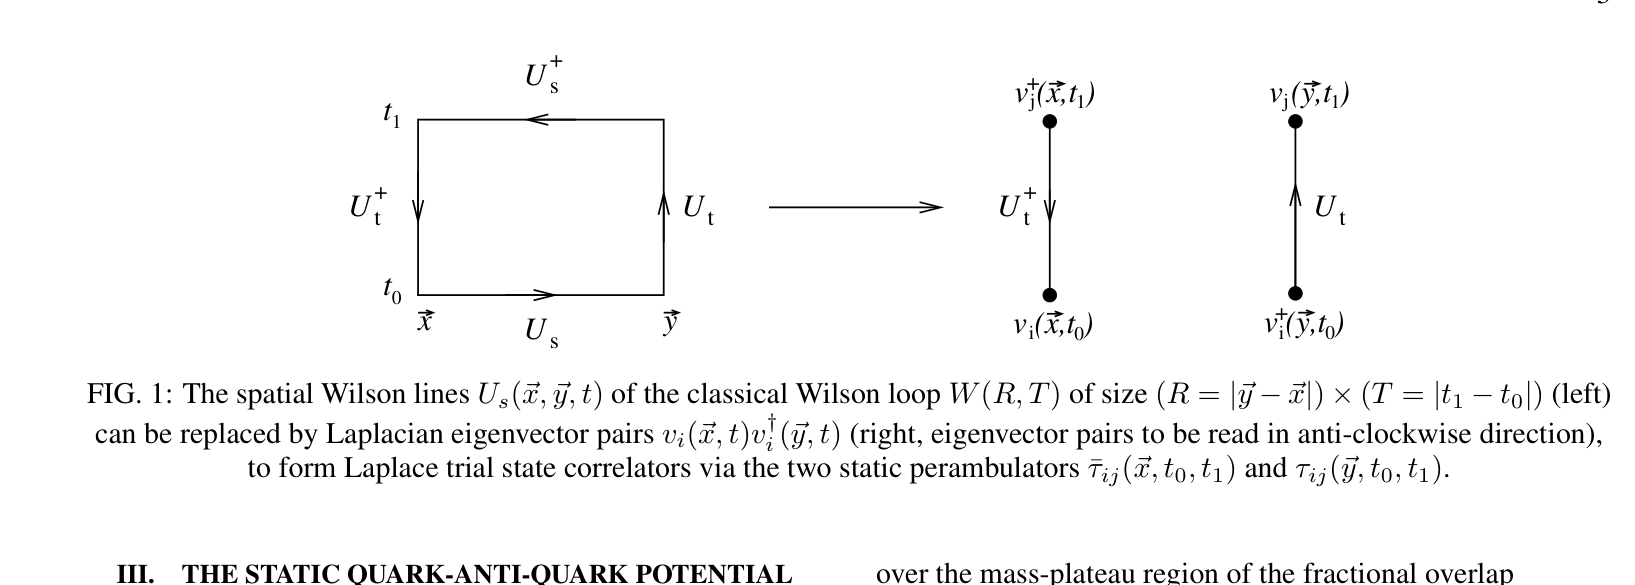
\includegraphics[height=0.27\textheight,width=\linewidth,keepaspectratio]{paper_laplace_wilson_replacement_fig1.png}
\end{column}
\begin{column}{0.46\textwidth}
\textbf{Analysis and statistics}\vspace{0.2em}
\begin{itemize}\tightitems
  \item Validate $L(R,\tau)$ via $V_{\rm eff}(R,\tau)$ and $V(R)$ before local-probe ratios.
  \item Action/energy density from $E^2$ and $B^2$ insertions.
  \item \texttt{pyerrors}/Gamma-method error analysis; jackknife cross-checks.
\end{itemize}
\vspace{1.08em}
{\tiny
\begin{tabular}{@{}p{0.18\linewidth}p{0.74\linewidth}@{}}
\toprule
2009 & Peardon et al.: distillation / Laplacian modes \\
2023 & H\"ollwieser et al.: static $Q\bar Q$ Laplace trial states \\
2005 & Bali et al.: string breaking and action-density profiles \\
2004--06 & Wolff: Gamma method for Monte Carlo errors \\
\bottomrule
\end{tabular}}
\end{column}
\end{columns}
\end{frame}

% ------------------------------------------------------------------
\begin{frame}{Current progress: from Laplace-static correlator to potential}
\scriptsize

\begin{columns}[T,totalwidth=\textwidth]

% ------------------------------------------------------------
\begin{column}{0.39\textwidth}

\textbf{Laplacian eigenmodes}\vspace{-0.2em}
\[
\Delta v_i = \lambda_i v_i,
\qquad i=1,\dots,N_v .
\]

\vspace{0.5em}
\textbf{Static perambulator}\vspace{-0.2em}
\[
 \tau_{ij}(\vec x;t_0,t_1)
 =
 v_i^\dagger(\vec x,t_0)\,
 U_t(\vec x;t_0,t_1)\,
 v_j(\vec x,t_1).
\]

\vspace{0.5em}
\textbf{Current profile choice}\vspace{-0.2em}
\[
\rho_i = 1,
\quad
i=1,\dots,N_v,
\quad
N_v=10 .
\]

\end{column}

% ------------------------------------------------------------
\begin{column}{0.51\textwidth}

\textbf{Laplace-static correlator}\vspace{-0.2em}
\[
 L(R,\tau)
 =
 \left\langle
 \sum_{i,j=1}^{N_v}
 \rho_i^2\rho_j^2\,
 \tau_{ij}(\vec y;t_0,t_1)\,
 \tau_{ji}(\vec x;t_1,t_0)
 \right\rangle ,
\]
\[
R=|\vec y-\vec x|,
\qquad
\tau=t_1-t_0 .
\]

\vspace{0.35em}
\textbf{Effective energy}\vspace{-0.2em}
\[
 V_{\rm eff}(R,T)
 =
 \log\frac{L(R,T)}{L(R,T+1)} .
\]

\vspace{0.35em}
\textbf{Cornell benchmark fit}\vspace{-0.2em}
\[
 aV(R)
 =
 aV_0+\sigma a^2 R-\frac{\alpha}{R}.
\]

\end{column}

\end{columns}

\vspace{0.35em}
\smallcite{Current tests: $N_v=10$ with constant eigenmode weights $\rho_i=1$; first validation through static-potential plateaus and Cornell fits.}

\end{frame}

% ------------------------------------------------------------------
\begin{frame}{Implementation status}
\begin{columns}[T,totalwidth=\textwidth]
\begin{column}{0.50\textwidth}
\textbf{Implemented code path}\vspace{0.2em}
\begin{itemize}\tightitems
  \item Read gauge fields and Laplacian eigenvectors from the existing QCD-library and HDF5 setup.
  \item Build $\tau_{ij}(\vec x,t_0,t_1)$ for each chosen $\tau=t_1-t_0$.
  \item Contract two static perambulators to form $L(R,\tau)$.
  \item Analyze $V_{\rm eff}$, plateau windows, and correlated fits.
\end{itemize}
\vspace{0.35em}
{\scriptsize Main compute test: \texttt{src/test\_laplace\_RT\_scan.c}.}
\end{column}
\begin{column}{0.46\textwidth}
\textbf{Current production setup}\vspace{0.2em}
\begin{itemize}\tightitems
  \item $N_{\rm cfg}=100$ gauge configurations.
  \item $N_v=10$ eigenvectors with constant weights $\rho_i=1$.
  \item Temporal-source average:
  $t_0=0,8,16,24,32,40$.
  \item Validated scan:
  $R/a=1\ldots 6$, $\tau/a=1\ldots 8$.
  \item Diagnostic scan:
  $R/a=1\ldots 12$, $\tau/a=1\ldots 10$.
\end{itemize}
\end{column}
\end{columns}
\end{frame}

% ------------------------------------------------------------------
\begin{frame}{Validation I: effective energies and plateau fits}
\begin{columns}[T,totalwidth=\textwidth]

% ------------------------------------------------------------
\begin{column}{0.66\textwidth}
\centering
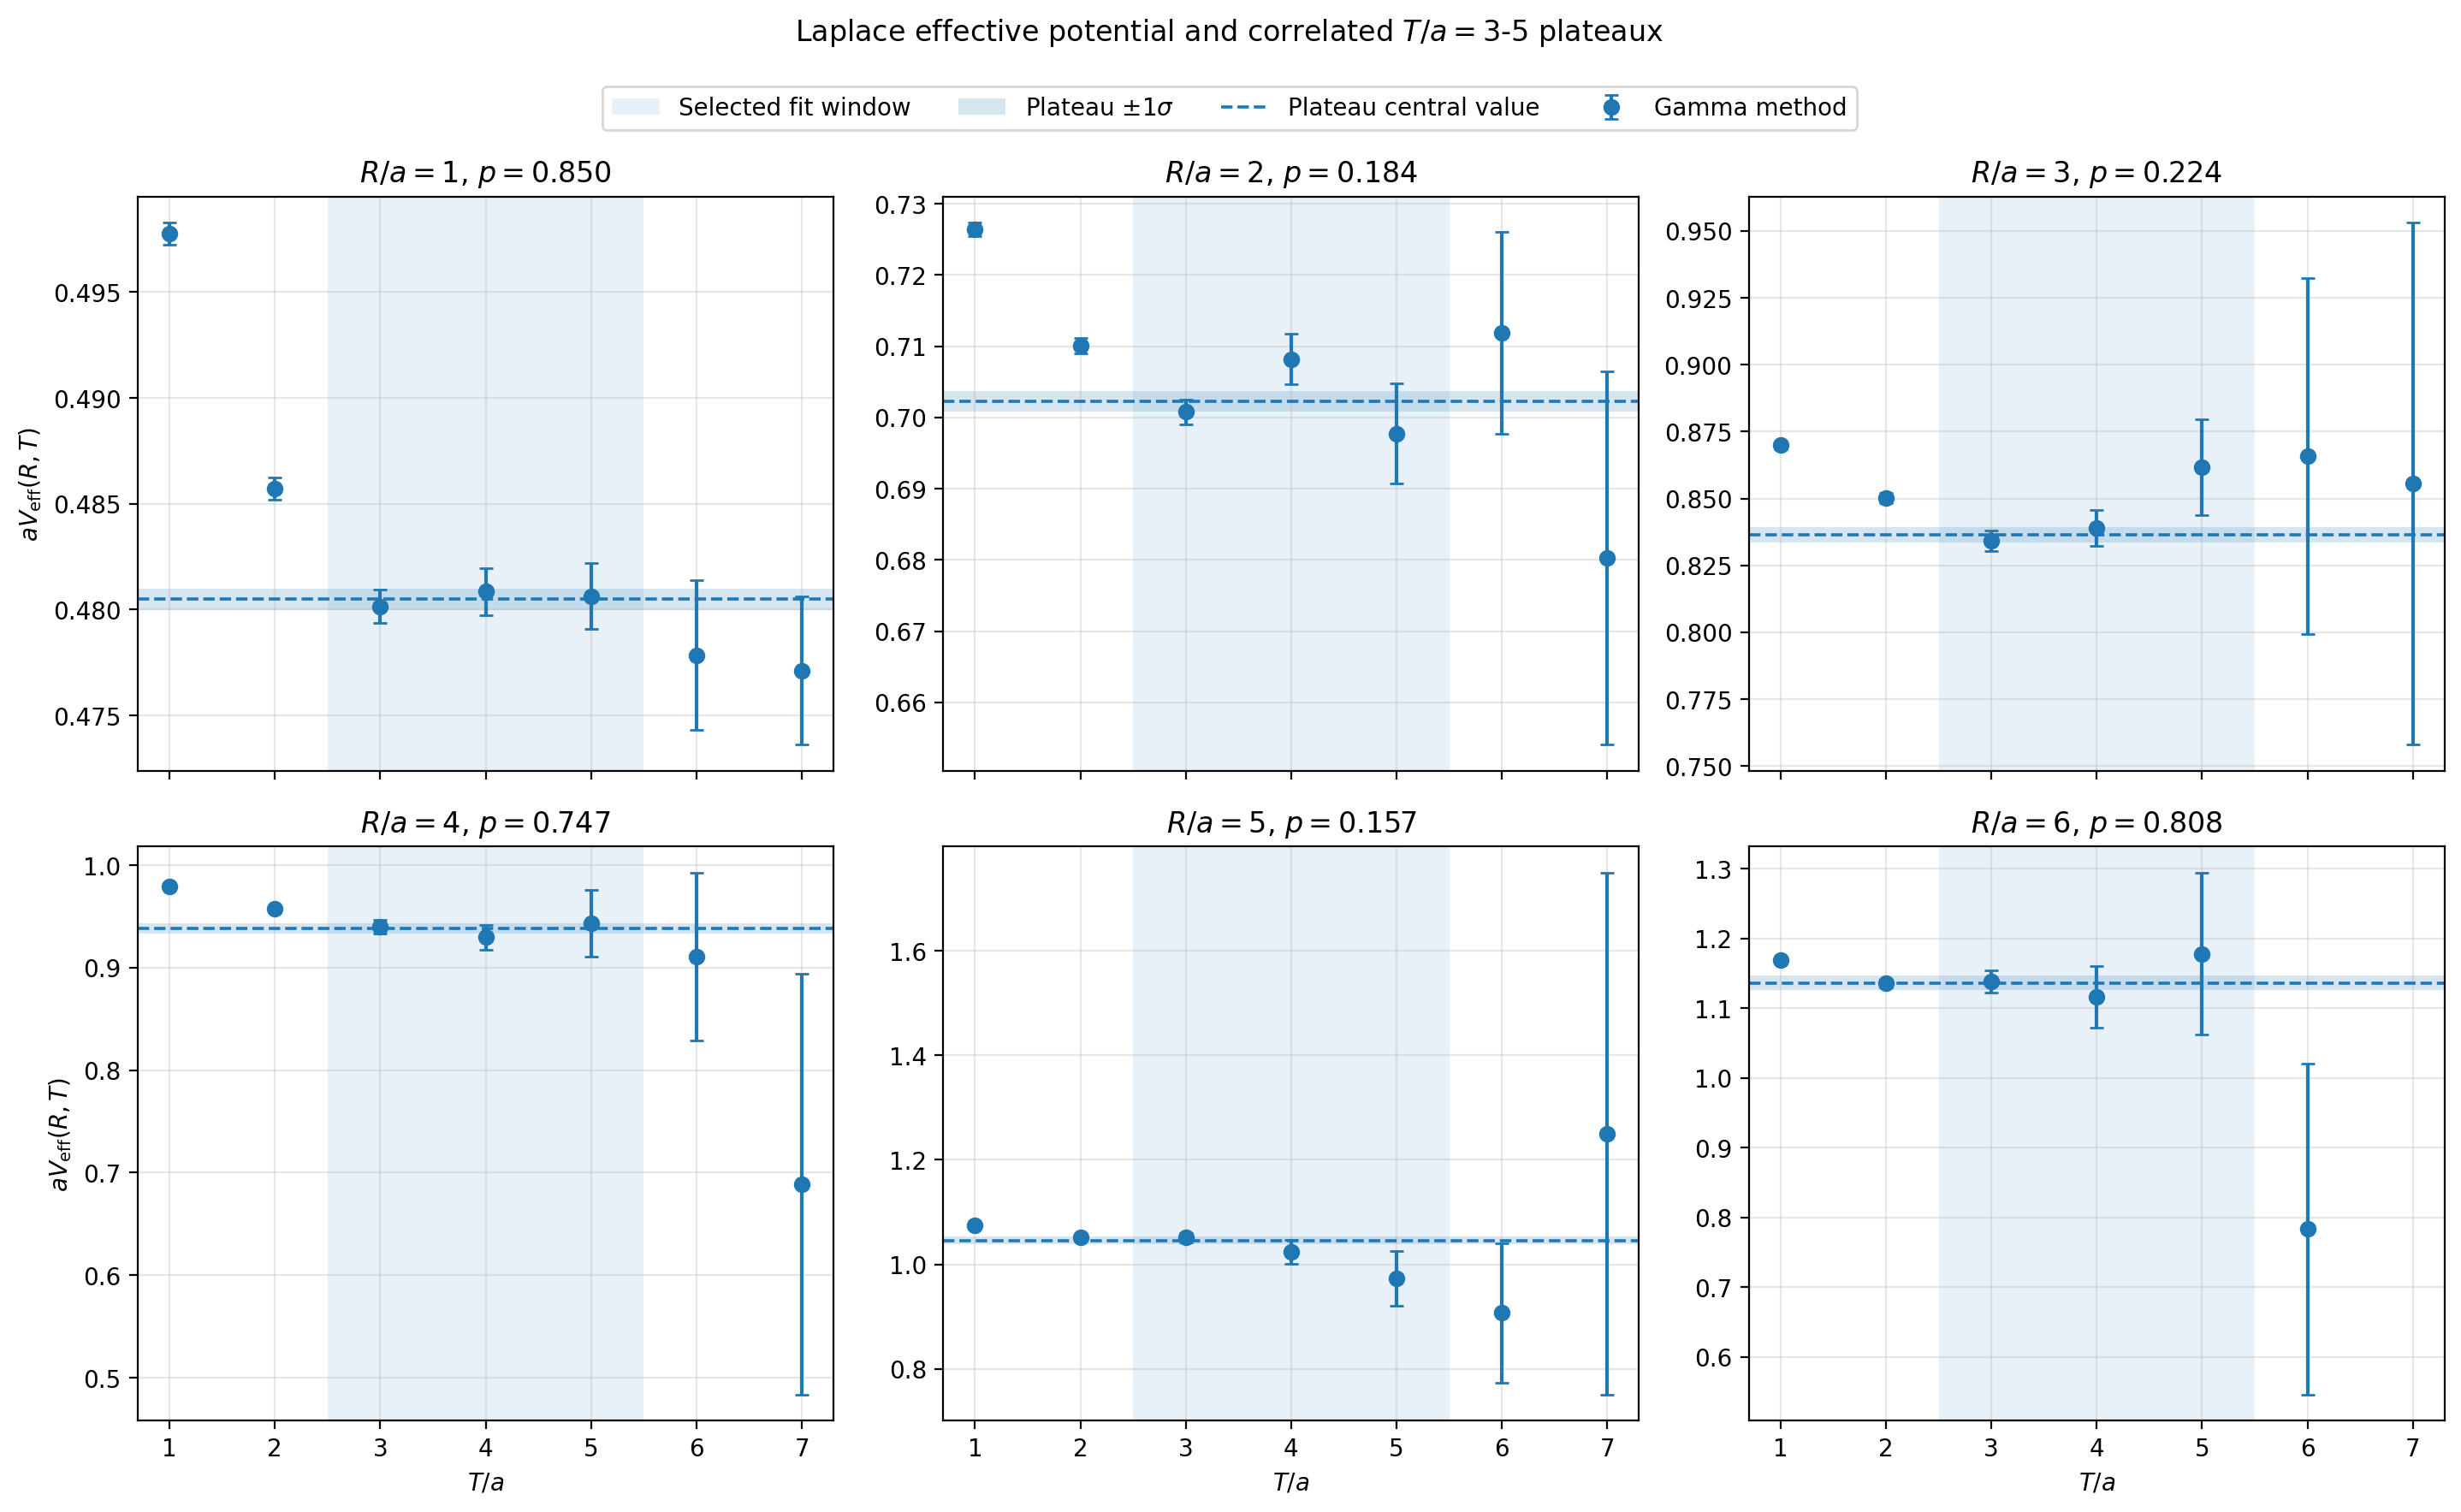
\includegraphics[width=\linewidth,keepaspectratio]{laplace_Veff_correlated_plateau_T3-5_t0avg6_R1-6.png}

\vspace{0.30em}
\begin{beamercolorbox}[rounded=true,sep=0.35em,wd=0.78\linewidth]{block body}
\centering
\scriptsize
\textbf{Takeaway:} source construction validated.\\[-0.01em]
Validated $L(R,\tau)$ normalizes the local-probe ratio:
\[
\Delta S_{Q\bar Q}
=
\frac{\langle L S\rangle}{\langle L\rangle}
-
\langle S\rangle .
\]
\end{beamercolorbox}
\end{column}

% ------------------------------------------------------------
\begin{column}{0.33\textwidth}
\textbf{Outcome}\vspace{0.2em}
\begin{itemize}\tightitems
  \item Validated region: $R/a=1\ldots6$.
  \item Stable plateau window: $\tau/a=3\ldots5$.
  \item Correlated constant fits give acceptable $\chi^2/{\rm dof}$ and $p$-values.
  \item Validated $L(R,\tau)$ normalizes the probe ratio.
\end{itemize}
\end{column}

\end{columns}
\end{frame}

% ------------------------------------------------------------------
\begin{frame}{Validation II: static potential and Cornell fit}
\begin{columns}[T,totalwidth=\textwidth]
\begin{column}{0.60\textwidth}
\centering
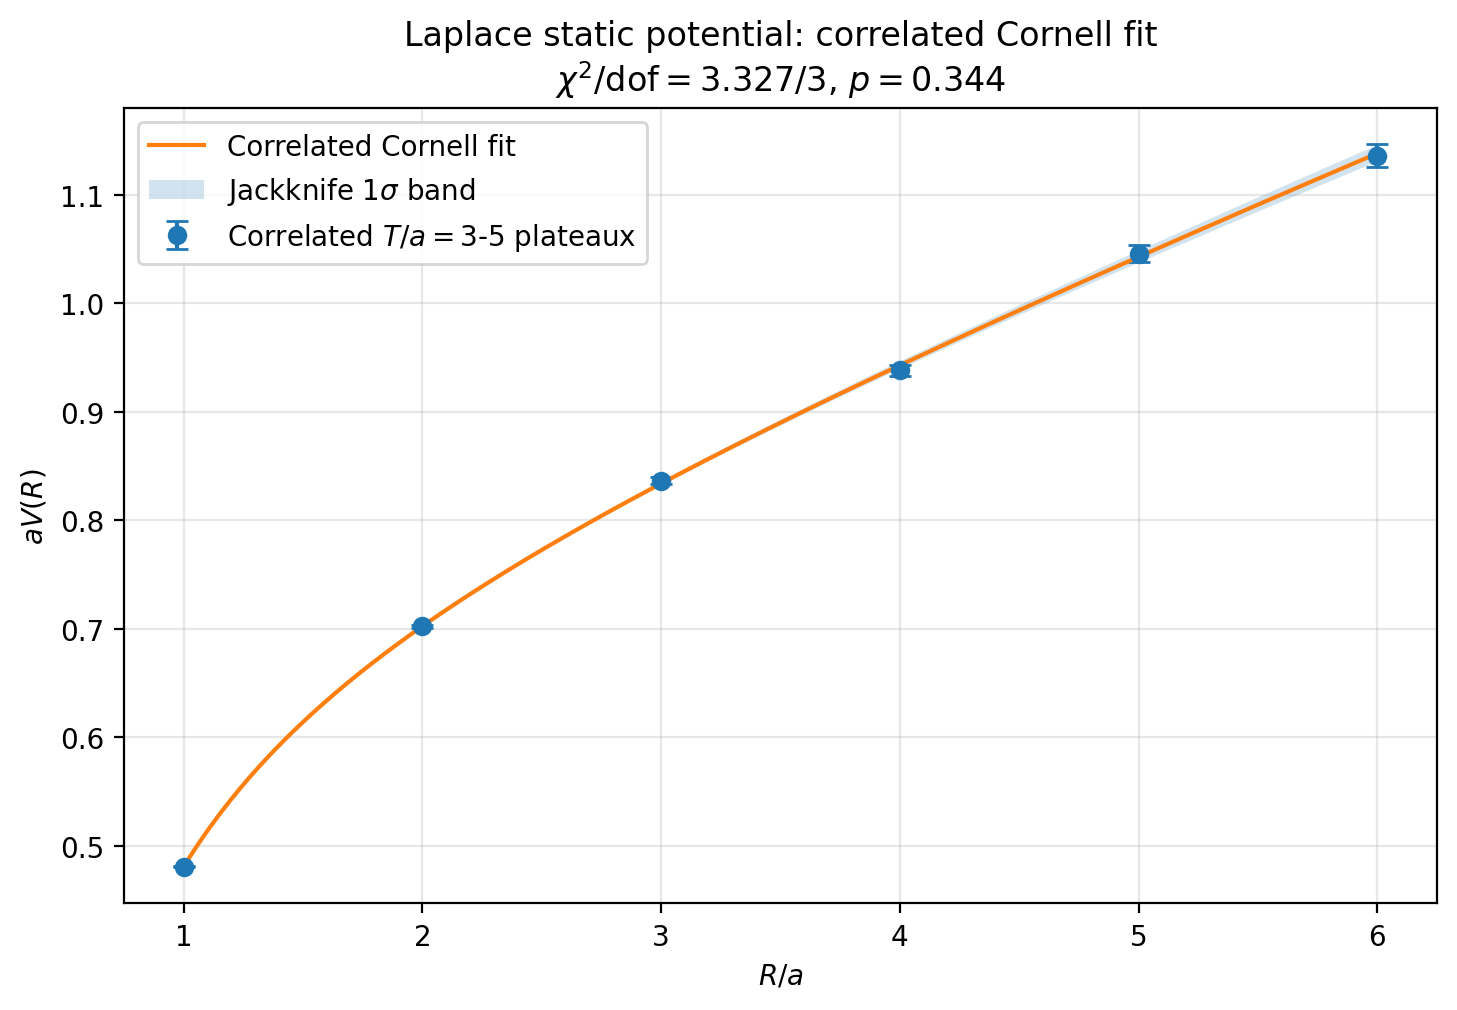
\includegraphics[height=0.62\textheight,width=\linewidth,keepaspectratio]{laplace_static_potential_cornell_R1-6_t0avg6.png}
\end{column}
\begin{column}{0.39\textwidth}
\textbf{Correlated Cornell fit}\vspace{-0.2em}
\begin{align*}
 aV(R)&=aV_0+\sigma a^2R-\frac{\alpha}{R},\\[-0.2em]
 \chi^2/{\rm dof}&=1.11,\quad p=0.344.
\end{align*}
\vspace{-0.2em}
{\scriptsize
\begin{tabular}{@{}ll@{}}
\toprule
$aV_0$ & $0.6646(82)$ \\
$\sigma a^2$ & $0.08646(24)$ \\
$\alpha$ & $0.2705(60)$ \\
$a\sqrt\sigma$ & $0.2940(40)$ \\
\bottomrule
\end{tabular}}
\vspace{0.35em}
\begingroup
\setlength{\leftmargini}{1.15em}
\begin{itemize}\tightitems
  \item Potential rises as expected.
  \item Fit stable under moderate range checks.
  \item Confirms expected static-potential behavior.
\end{itemize}
\endgroup
\end{column}
\end{columns}
\end{frame}

% ------------------------------------------------------------------
% ------------------------------------------------------------------
\begin{frame}{Reliability diagnostics for the extended scan}

\begin{columns}[T,totalwidth=\textwidth]
\begin{column}{0.33\textwidth}
\centering
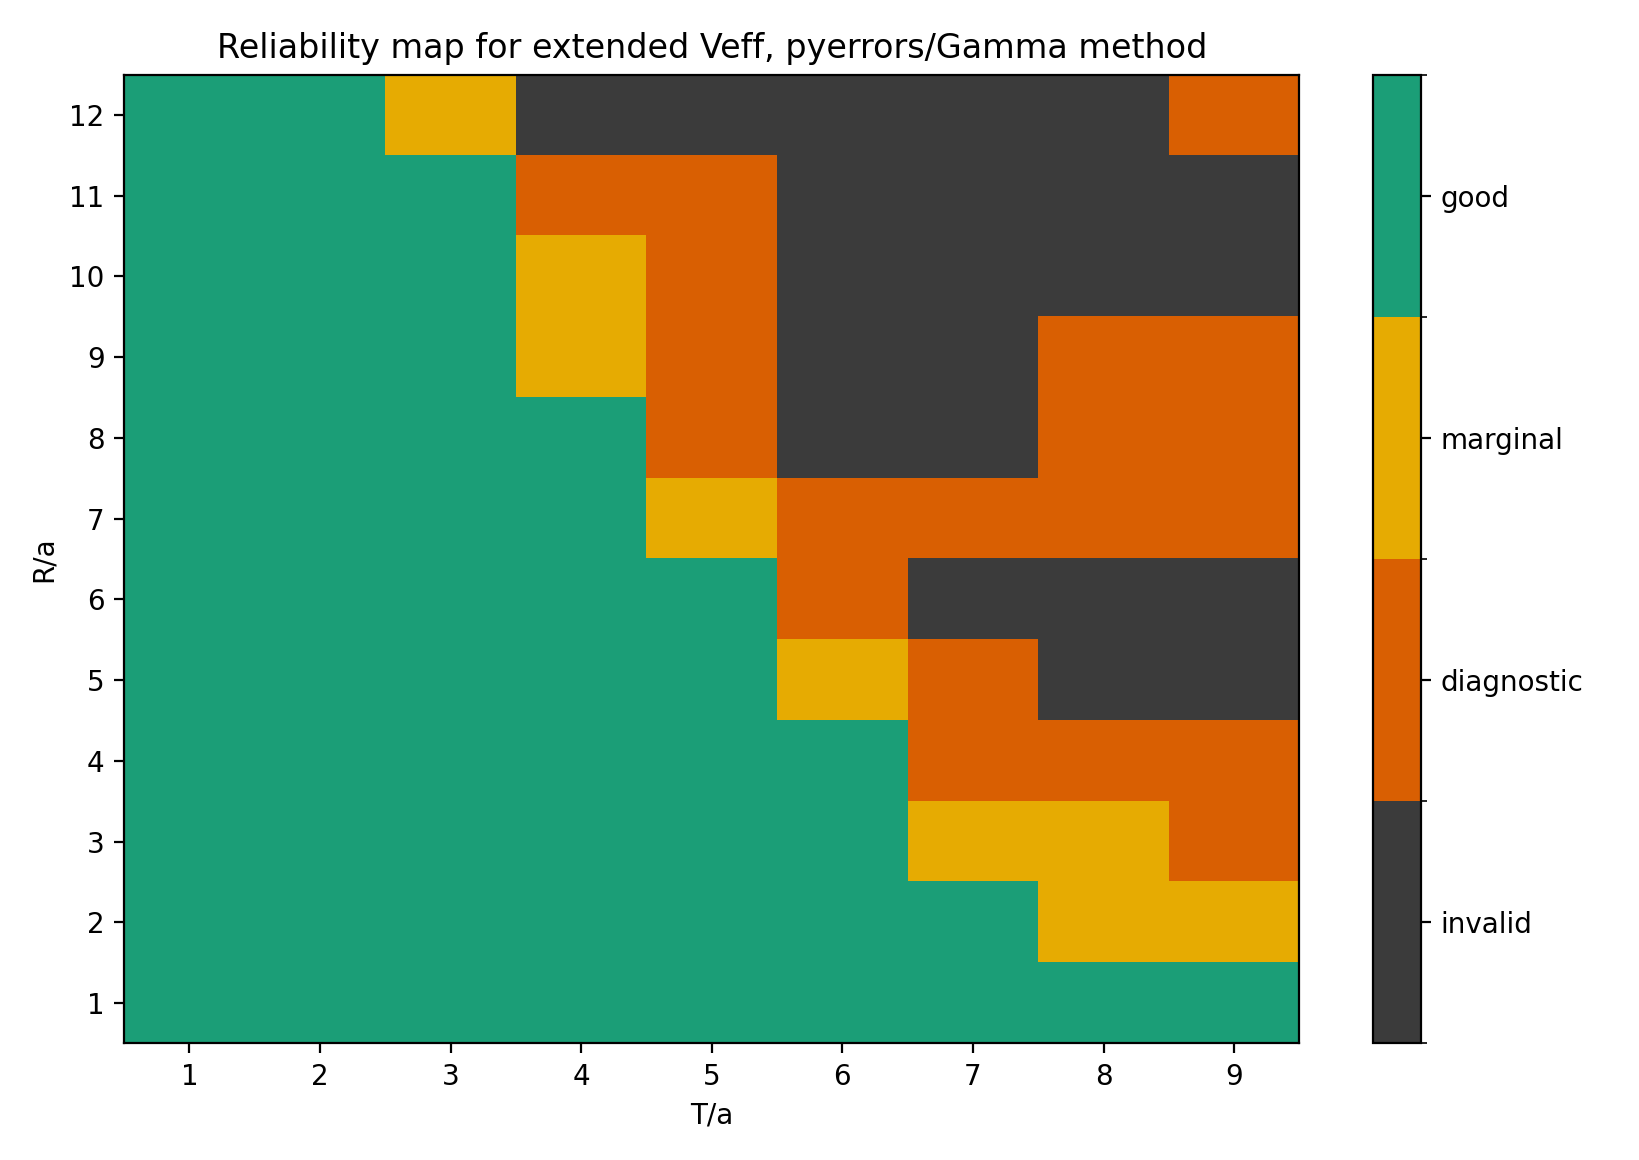
\includegraphics[height=0.47\textheight,width=\linewidth,keepaspectratio]{laplace_reliability_map_t0avg6_R12T10.png}

\vspace{0.15em}
{\scriptsize\textbf{Reliability map}\\
combined quality class}
\end{column}

\begin{column}{0.33\textwidth}
\centering
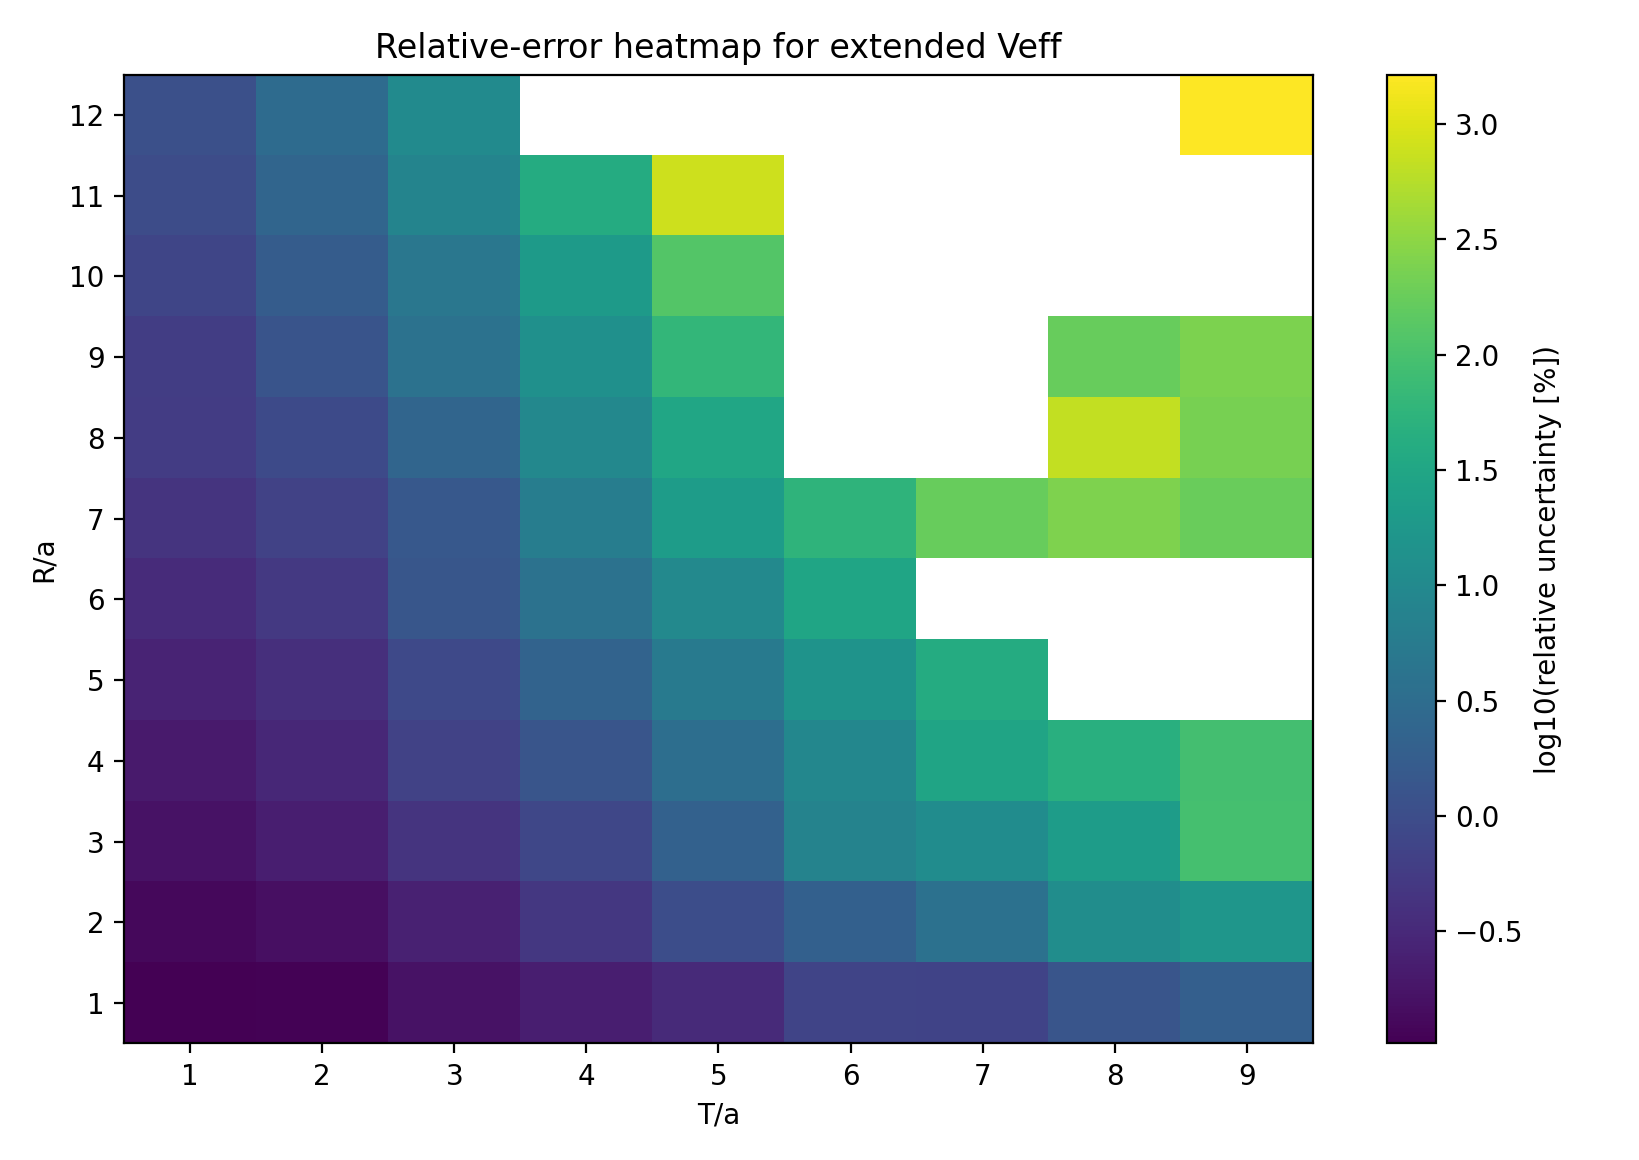
\includegraphics[height=0.47\textheight,width=\linewidth,keepaspectratio]{laplace_relative_error_heatmap_t0avg6_R12T10.png}

\vspace{0.15em}
{\scriptsize\textbf{Relative uncertainty}\\
statistical noise level}
\end{column}

\begin{column}{0.33\textwidth}
\centering
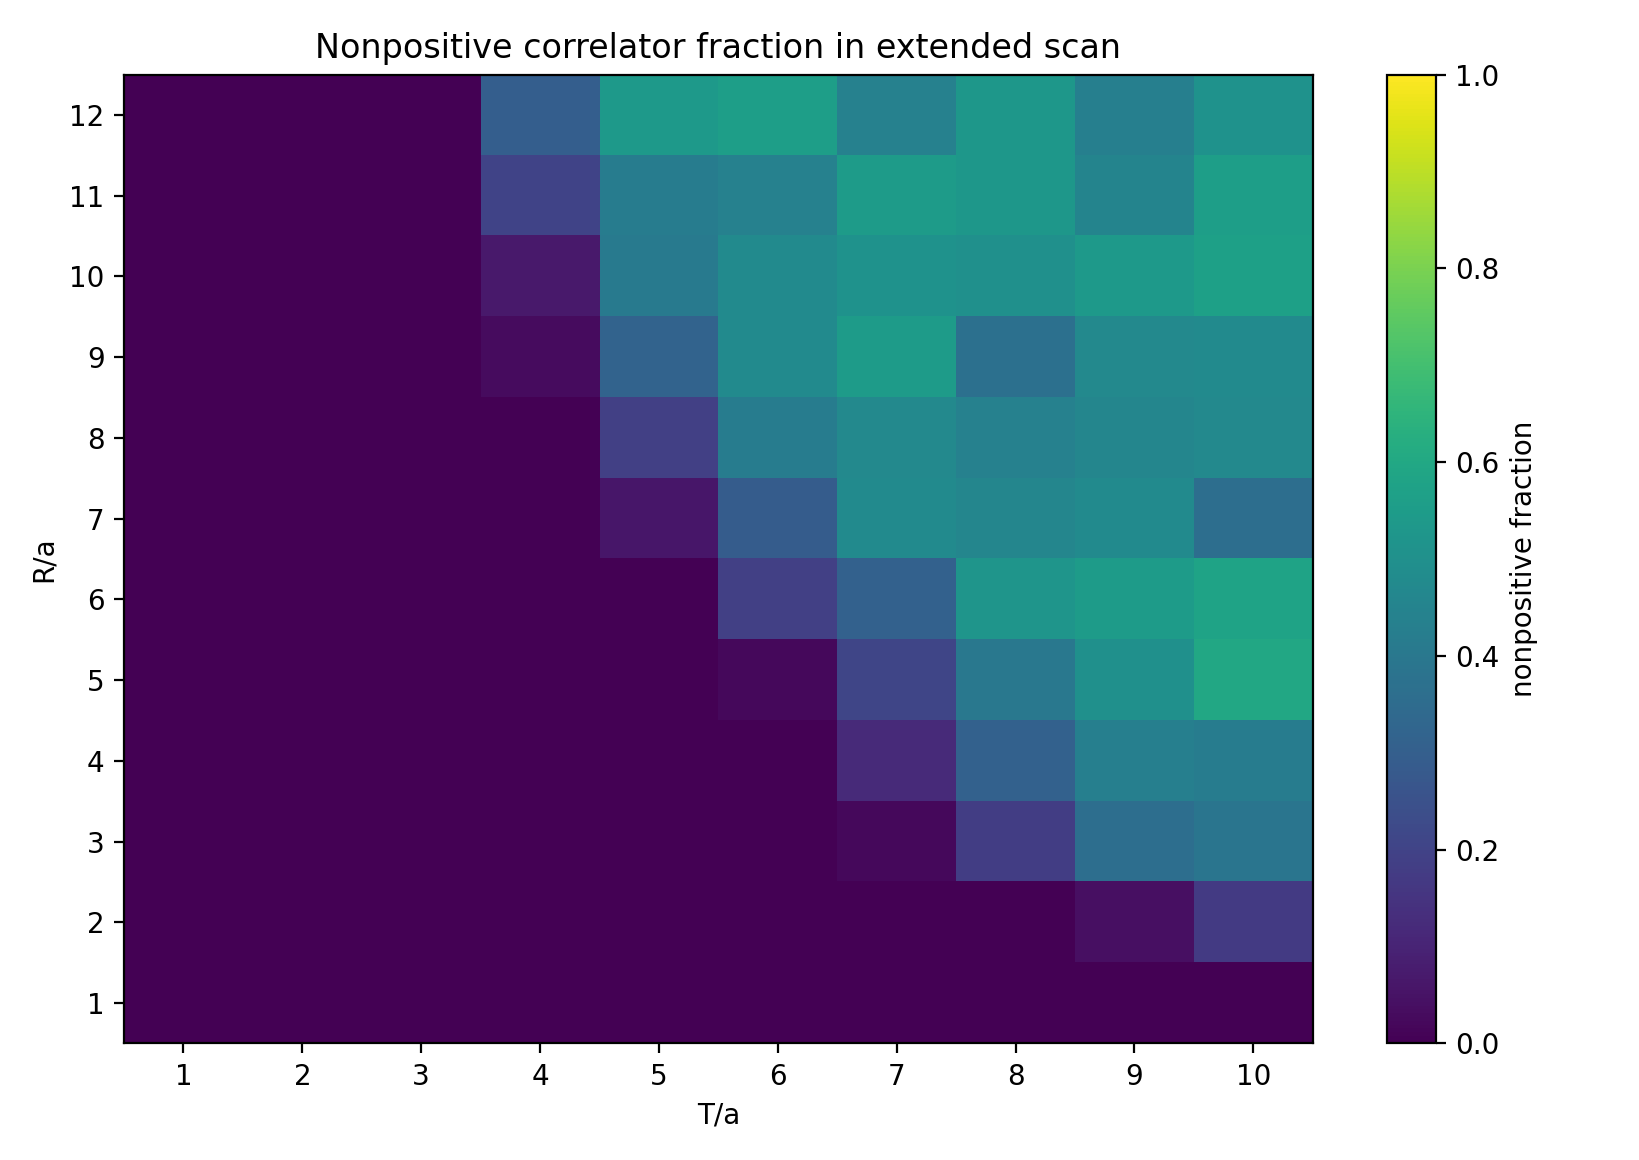
\includegraphics[height=0.47\textheight,width=\linewidth,keepaspectratio]{laplace_nonpositive_fraction_heatmap_t0avg6_R12T10.png}

\vspace{0.15em}
{\scriptsize\textbf{Non-positive fraction}\\
sign/log stability check}
\end{column}
\end{columns}

\vspace{0.99em}

\begin{minipage}{\textwidth}
\centering
\begin{beamercolorbox}[rounded=true,sep=0.45em,wd=0.86\textwidth]{block body}
\scriptsize
\begin{minipage}[t]{0.28\linewidth}
\raggedright
\textcolor{green!45!black}{\textbf{Good}}\\[0.15em]
low uncertainty; positive samples
\end{minipage}
\hfill
\begin{minipage}[t]{0.28\linewidth}
\raggedright
\textcolor{orange!85!black}{\textbf{Marginal}}\\[0.15em]
usable mainly for trend checks
\end{minipage}
\hfill
\begin{minipage}[t]{0.31\linewidth}
\raggedright
\textcolor{gray!70!black}{\textbf{Diagnostic/invalid}}\\[0.15em]
large uncertainty or sign problems
\end{minipage}
\end{beamercolorbox}

\vspace{0.22em}

{\scriptsize
The extended scan is used to select safe parameter windows for the first flux-tube probe measurements.
}
\end{minipage}

\end{frame}

% ------------------------------------------------------------------
\begin{frame}{Extended-distance diagnostic scan}
\begin{columns}[T,totalwidth=\textwidth]
\begin{column}{0.63\textwidth}
\centering
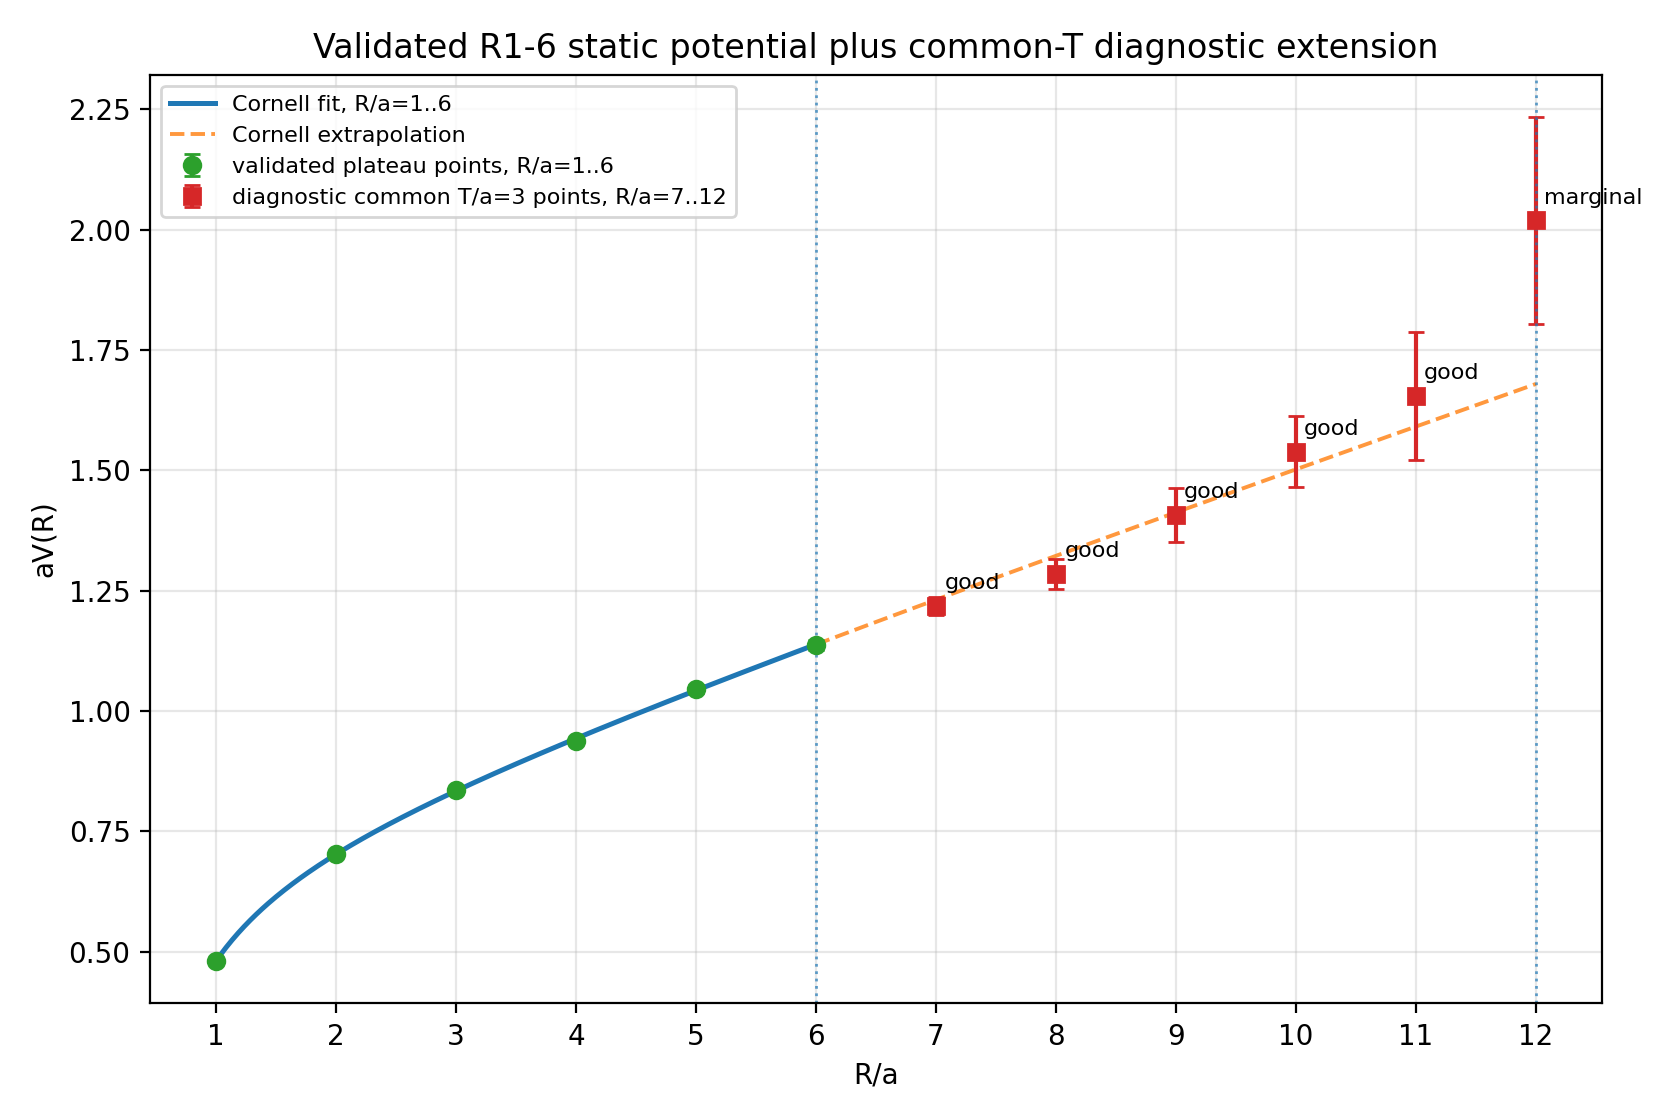
\includegraphics[height=0.61\textheight,width=\linewidth,keepaspectratio]{laplace_static_potential_R1-6_fit_plus_R7-12_commonT3_diagnostic_t0avg6.png}

\vspace{0.25em}
{\scriptsize Red points indicate a common $\tau/a=3$ diagnostic estimate beyond the validated fit range.}
\end{column}
\begin{column}{0.33\textwidth}
\textbf{What this tells us}\vspace{0.2em}
\begin{itemize}\tightitems
  \item Extended scan reproduces the validated $R/a=1\ldots6$ region.
  \item $R/a=7,8$ show selected plateau-like windows.
  \item Larger $R/a$ values remain diagnostic with the current statistics/profile.
\end{itemize}

\end{column}
\end{columns}
\end{frame}

% ------------------------------------------------------------------
\begin{frame}{Next step: local gluonic density insertion}
\footnotesize
\begin{columns}[T,totalwidth=\textwidth]

% ------------------------------------------------------------
\begin{column}{0.48\textwidth}
\textbf{Field-strength probe}\vspace{0.01em}

{\scriptsize
\[
F_{\mu\nu}(x)\leftarrow \text{clover/plaquette estimator}
\]
\vspace{-0.9em}

\centering
from oriented $\mu\nu$ loops.
}

\vspace{0.35em}
{\scriptsize
\[
\begin{aligned}
E^2(\vec z,t)
&=
\sum_{i=1}^{3}
{\rm Tr}\,\big[F_{i t}(\vec z,t)^2\big],\\[0.25em]
B^2(\vec z,t)
&=
\sum_{i<j}
{\rm Tr}\,\big[F_{ij}(\vec z,t)^2\big],\\[0.25em]
S(\vec z,t)
&=
\frac12\left(E^2(\vec z,t)+B^2(\vec z,t)\right).
\end{aligned}
\]
}

\vspace{0.55em}
\textbf{Physical question}\vspace{0.25em}

{\scriptsize
How is the local gluonic density modified by a static
$Q\bar Q$ pair separated by $R$?
}

\end{column}

% ------------------------------------------------------------
\begin{column}{0.48\textwidth}
\textbf{Normalized and vacuum-subtracted profile}\vspace{0.01em}

{\scriptsize
\[
\begin{aligned}
C_L(R,\tau)
&\equiv
\langle L(R,\tau)\rangle,\\[0.25em]
C_{LS}(\vec z;R,\tau)
&\equiv
\left\langle
L(R,\tau)\,
S(\vec z,t_{\rm mid})
\right\rangle .
\end{aligned}
\]
}

\vspace{0.15em}
{\scriptsize
\[
\Delta S(\vec z;R,\tau)
=
\frac{C_{LS}(\vec z;R,\tau)}
     {C_L(R,\tau)}
-
\left\langle S(\vec z,t_{\rm mid})\right\rangle .
\]
}

\vspace{0.55em}
\textbf{Prototype choices}\vspace{0.2em}

\begin{itemize}\tightitems
  \item insert probe at $t_{\rm mid}=t_0+\tau/2$ where possible
  \item first source pair: on-axis $R/a=3$ or $4$
  \item start with $S$, then analyze $E^2$ and $B^2$ separately
\end{itemize}

\end{column}

\end{columns}
\end{frame}

% ------------------------------------------------------------------
\begin{frame}{Near-term plan for flux-tube profiles}
\begin{columns}[T,totalwidth=\textwidth]

\begin{column}{0.47\textwidth}
\textbf{Immediate prototype}\vspace{0.2em}

\begin{enumerate}\setlength\itemsep{0.35em}
  \item Reuse the validated $L(R,\tau)$ pipeline and temporal source averaging.
  \item Insert local $S(\vec z,t_{\rm mid})$ using qcdlib field-strength routines.
  \item Accumulate $\langle LS\rangle$, $\langle L\rangle$, and $\langle S\rangle$ in one pass.
  \item First output a 2D mid-plane map; then generalize to full 3D HDF5 data.
\end{enumerate}

\vspace{0.35em}
{\scriptsize
First target: on-axis $R/a=3$ or $4$ in the validated plateau window.
}
\end{column}

\begin{column}{0.49\textwidth}
\centering
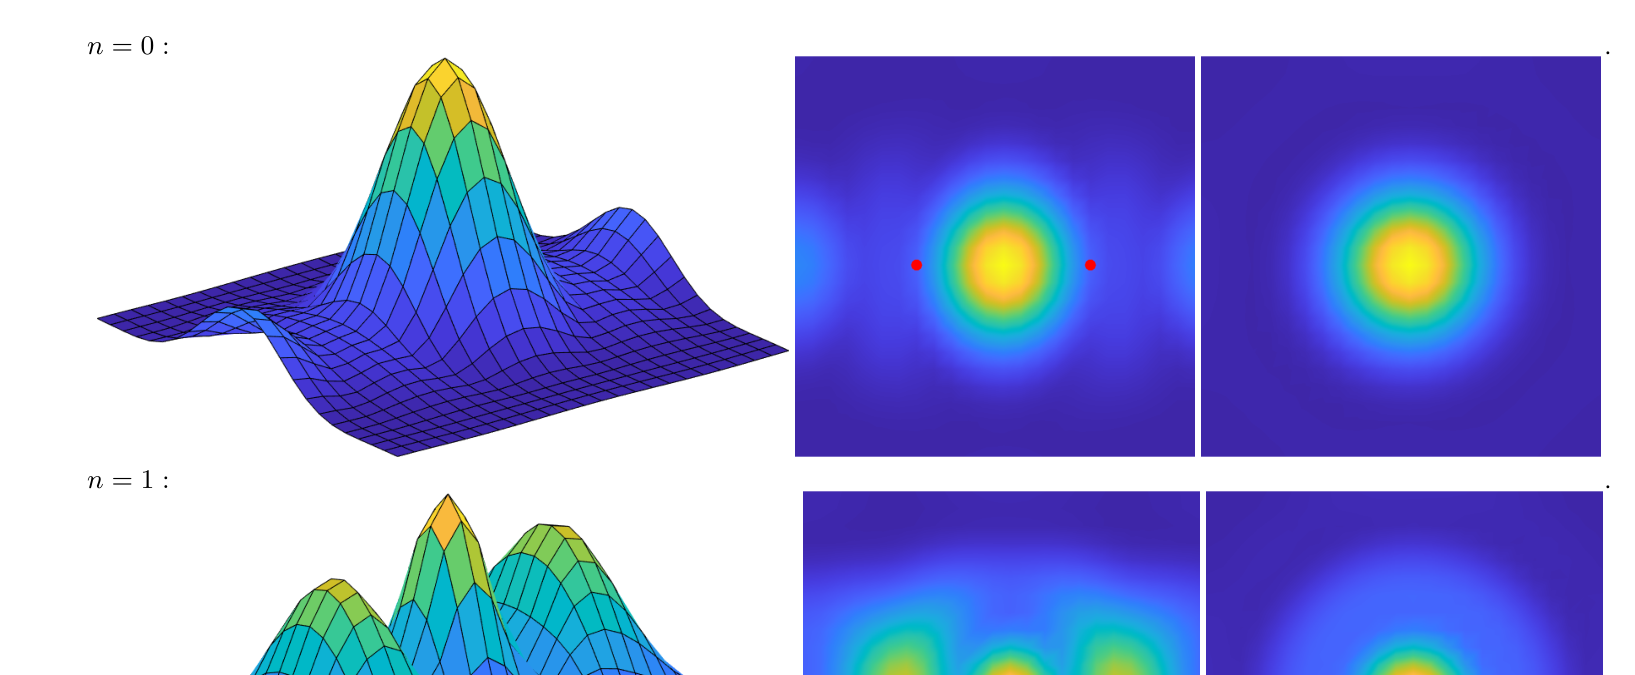
\includegraphics[height=0.43\textheight,width=\linewidth,keepaspectratio]{paper_laplace_spatial_distribution_fig7.png}

\vspace{0.27em}
\smallcite{Analogy from Laplace trial-state profiles: later we aim to map local gluonic density instead.}

\vspace{1.11em}
\makebox[\linewidth][r]{%
\begin{beamercolorbox}[rounded=true,sep=0.45em,wd=0.86\linewidth]{block body}
\centering
\scriptsize
First physics map: $\Delta S(\vec z;R,\tau)$.\\[0.25em]
Later: $\Delta E^2$, $\Delta B^2$, smeared probes, and orientation averaging.
\end{beamercolorbox}%
}
\end{column}

\end{columns}
\end{frame}

% ------------------------------------------------------------------
\begin{frame}{Status summary: validated source and next probes}
\begin{columns}[T,totalwidth=\textwidth]

\begin{column}{0.49\textwidth}
\textbf{Validated baseline}\vspace{0.2em}
\begin{itemize}\tightitems
  \item Static perambulator and Laplace-static correlator pipeline is working.
  \item Six temporal-source averaging is implemented.
  \item $R/a=1\ldots6$ potential extraction is validated with correlated plateau fits.
  \item Cornell benchmark gives a physically sensible and statistically acceptable potential.
\end{itemize}
\end{column}

\begin{column}{0.48\textwidth}
\textbf{Next implementation step}\vspace{0.2em}
\begin{itemize}\tightitems
  \item $R/a=7\ldots12$ scan is useful diagnostically, but not yet final physics.
  \item Flux-tube profiles require inserting a local field-strength probe.
  \item First target: $\Delta S(\vec z;R,\tau)$ for on-axis $R/a=3$ or $4$.
  \item Open choices: probe smearing, orientation averaging, and statistics.
\end{itemize}

\vspace{0.21em}
\begin{beamercolorbox}[rounded=true,sep=0.45em,wd=0.92\linewidth]{block body}
\centering
\scriptsize
Current stage: static-source validation is complete; implementation now moves to local gluonic-density probes.
\end{beamercolorbox}
\end{column}

\end{columns}
\end{frame}

% ------------------------------------------------------------------
\backupslidetrue
\begin{frame}[fragile,noframenumbering]{Backup: selected files and commands to show}
\tiny
\begin{tabular}{@{}p{0.25\linewidth}p{0.66\linewidth}@{}}
\toprule
Purpose & File / result \\
\midrule
Code & \texttt{src/test\_laplace\_RT\_scan.c} \\
Plateaux & \texttt{laplace\_Veff\_correlated\_plateau\_T3-5\_t0avg6\_R1-6.png} \\
Cornell fit & \texttt{laplace\_static\_potential\_cornell\_R1-6\_t0avg6.png} \\
Reliability map & \texttt{laplace\_reliability\_map\_t0avg6\_R12T10.png} \\
Diagnostic extension & \texttt{laplace\_static\_potential\_R1-6\_fit\_plus\_R7-12\_...png} \\
R7/R8 window check & \texttt{laplace\_plateau\_window\_comparison\_R7\_R8\_...png} \\
\bottomrule
\end{tabular}
\vspace{2.7em}

\textbf{Results and plots location on Stromboli}\vspace{-0.9em}
\begin{verbatim}
cd /home/m2130292/Masterarbeit/laplace_static
ls -lh results/figures/*t0avg6*.png | head
\end{verbatim}
\end{frame}
\backupslidefalse

\end{document}
